% -*- LaTeX -*-
% -*- coding: utf-8 -*-
%
% michael a.g. aïvázis
% california institute of technology
% (c) 1998-2012 all rights reserved
%

\lecture{Programming with pthreads - part 2}{20120125}

% --------------------------------------
% hello world
\begin{frame}[fragile]
%
  \frametitle{Hello world}
  \label{slide:hello-world-threads}
%
  \begin{C}
#include <pthread.h>
#include <stdio.h>
#define THREADS 10

void* hello(void* threadID) {
    long id = (long) threadID;
    printf("hello from %02ld/%0d\n", id, THREADS);
    pthread_exit(NULL);
    return NULL;
}

int main(int argc, char* argv[]) {
    long id;
    int status;
    pthread_t threads[THREADS];

    for (id=0; id<THREADS; id++) {
        printf("creating thread %02ld\n", id);
        status = pthread_create(&threads[id], NULL, hello, (void*) id);
        if (status) {
            printf("error %d in pthread_create\n", status);
        }
    }
    /* there is a problem here... */
    pthread_exit(NULL);
    return 0;
}
  \end{C}
%
\end{frame}

% --------------------------------------
% joining and detaching threads
\begin{frame}[fragile]
%
  \frametitle{Joining and detaching}
%
  \begin{itemize}
%
  \item in the example in \slideref{hello-world-threads}, the main thread exits without knowing whether
    any of the threads it spawned have finished
    \begin{itemize}
    \item saying ``hello'' is asynchronous
    \item but gathering the results of parallel calculations normally isn't
    \end{itemize}
%
  \item {\em thread synchronization} can be achieved using \function{pthread\_join}
    \begin{itemize}
      \item the \function{pthread\_create} caller saves the thread id
      \item the thread is scheduled, executes, and calls \function{pthread\_exit}
      \item any other thread can wait for this thread to finish by calling
        \function{pthread\_join} with the saved thread id and also retrieve the termination
        status
    \end{itemize}
%
  \item for this to work, a thread must be {\em joinable}
    \begin{itemize}
    \item controlled by the thread creation attributes
    \item for portability, you should always mark your joinable threads explicitly
    \end{itemize}
%
%
    \item a thread that will never be joined may be {\em detached}
      \begin{itemize}
      \item by setting the corresponding attribute during thread creation
      \item or, by calling \function{pthread\_detach} at any point
      \item detaching a thread saves some system resources
      \end{itemize}
        
  \end{itemize}
%
\end{frame}

% --------------------------------------
% mutexes
\begin{frame}[fragile]
%
  \frametitle{Creating mutexes}
%
  \begin{itemize}
%
  \item a {\em mutex} is a locking mechanism that helps guarantee exclusive access to a section
    of code, most often to control access to shared variables
%
  \item mutexes are created using
%
    \begin{C}
int pthread_mutex_init(
    pthread_mutex_t* mutex, const pthread_mutexattr_t* attr);
    \end{C}
%
    \begin{itemize}
    \item they start out unlocked
    \item the \identifier{attr} enables more advanced (but perhaps non-portable) use
    \end{itemize}
%
  \item mutexes are destroyed using
%
    \begin{C}
int pthread_mutex_destroy(pthread_mutex_t* mutex);
    \end{C}
%
    \begin{itemize}
    \item destroy mutexes you are no longer using to prevent resource leakage
    \end{itemize}
%
  \end{itemize}
%
\end{frame}

% --------------------------------------
% mutex manipulation
\begin{frame}[fragile]
%
  \frametitle{Locking and unlocking mutexes}
%
  \begin{itemize}
%
  \item threads manipulate mutexes through
%
    \begin{C}
int pthread_mutex_lock(pthread_mutex_t* mutex);
int pthread_mutex_trylock(pthread_mutex_t* mutex);
int pthread_mutex_unlock(pthread_mutex_t* mutex);
    \end{C}
%
  \item \identifier{pthread\_mutex\_lock} attempts to gain exclusive access
    \begin{itemize}
    \item if the mutex is unlocked, it locks it and returns
    \item otherwise, it blocks until the mutex is unlocked; when the mutex is unlocked, it
      locks it and returns
    \end{itemize}
%
  \item \identifier{pthread\_mutex\_unlock} attempts to release a mutex
    \begin{itemize}
    \item if it was previously locked by this thread, the mutex is unlocked
    \item if it was not previously locked, the call returns with an error code
    \item if it was locked, but not by the calling thread, the call returns an error code
    \end{itemize}
%
  \item \identifier{pthread\_mutex\_trylock} attempts to lock the mutex
    \begin{itemize}
    \item if it is unlocked, the call locks it and returns
    \item if it is locked, the call returns immediately with a {\em busy} error code
    \end{itemize}
%
  \item locking and unlocking mutexes is explicitly orchestrated by the programmer
  \item when multiple threads are blocked waiting for a mutex, there is no way to predict which
    one will succeed when the mutex becomes available
%
  \end{itemize}
%
\end{frame}


% --------------------------------------
% reduction using shared memory
\begin{frame}[fragile]
%
  \frametitle{Reduction on a shared memory machine}
%
%
  \begin{figure}
    \centering
    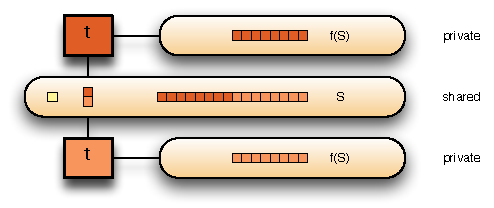
\includegraphics[width=\linewidth]{figures/threads-reduction.pdf}
    \label{fig:reduction-shared}
  \end{figure}
%
\end{frame}

% --------------------------------------
% sum of squares
\begin{frame}[fragile]
%
  \frametitle{Example reduction using threads}
  \label{slide:squares-threads}
%
  \begin{C}[basicstyle=\tt\bfseries\tiny]
#include <pthread.h>
#include <stdio.h>
#define THREADS 10
/* global variables -- yuck! */
long sum = 0;
pthread_mutex_t mutex;
/* worker */
void* squares(void* threadID) {
    long id = (long) threadID;
    pthread_mutex_lock(&mutex);
    sum += id*id;
    pthread_mutex_unlock(&mutex);
    pthread_exit(NULL);
    return NULL;
}
/* main program */
int main(int argc, char* argv[]) {
    long id;
    pthread_t threads[THREADS];
    pthread_mutex_init(&mutex, NULL);
    /* create some threads */
    for (id=0; id<THREADS; id++) {
        pthread_create(&threads[id], NULL, squares, (void*) id);
    }
    /* wait for them  to finish */
    for (id=0; id<THREADS; id++) {
        pthread_join(threads[id], NULL);
    }
    /* print the result */
    printf("sum = %ld\n", sum);
    /* exit */
    pthread_exit(NULL);
    return 0;
}
  \end{C}
%
\end{frame}

% --------------------------------------
% condition variables
\begin{frame}[fragile]
%
  \frametitle{Condition variables}
%
  \begin{itemize}
%
  \item condition variables build upon mutexes to enable threads to signal each other when some
    condition is met
%
  \item they are created using
%
    \begin{C}
int pthread_cond_init(
    pthread_cond_t* condition, const pthread_condattr_t* attr);
    \end{C}
%
  \item and destroyed using
%
    \begin{C}
int pthread_cond_destroy(pthread_cond_t* condition);
    \end{C}
%
  \end{itemize}
%
\end{frame}

% --------------------------------------
% using condition variables
\begin{frame}[fragile]
%
  \frametitle{Using condition variables}
%
  \begin{itemize}
%
  \item the following three routines implement the condition variable semantics
%
    \begin{C}
int pthread_cond_wait(pthread_cond_t* cond, pthread_mutex_t* mutex);
int pthread_cond_signal(pthread_cond_t* cond);
int pthread_cond_broadcast(pthread_cond_t* cond);
    \end{C}
%
  \item \identifier{pthread\_cond\_wait} blocks the calling thread until the specified
    condition is {\em signaled}
    \begin{itemize}
    \item it must be called with the mutex locked by the calling thread
    \item \identifier{pthread\_cond\_wait} releases the lock while the thread is blocked
    \item after the matching signal is received, the thread is awakened and the mutex locked
    \item the thread is responsible for releasing the mutex when it is done
    \end{itemize}
%
  \item \identifier{pthread\_cond\_signal} wakes up a thread that is waiting for the given
    condition variable
    \begin{itemize}
    \item mutex must be locked before calling it
    \item mutex must be unlocked after signaling, so blocking threads can be awakened
    \end{itemize}
%
  \item \identifier{pthread\_cond\_broadcast} can be used instead if multiple threads are
    waiting for a signal
%
  \end{itemize}
%
\end{frame}

% --------------------------------------
% condition variable caveats
\begin{frame}[fragile]
%
  \frametitle{Condition variable caveats}
%
  \begin{itemize}
%
  \item be careful with condition variables; make sure that
    \begin{itemize}
    \item a thread has called \identifier{pthread\_cond\_wait} before any thread
      calls \identifier{pthread\_cond\_signal}
    \item the mutex associated with the condition is locked before calling
      \identifier{pthread\_cond\_wait}, otherwise it might {\em not block}
    \item the thread that calls \identifier{pthread\_cond\_signal} unlocks the associated
      mutex, otherwise the threads waiting for the signal will continue to block
    \end{itemize}
%
%
  \end{itemize}
%
\end{frame}

% --------------------------------------
% the attribute interface
\begin{frame}[fragile]
%
  \frametitle{Attributes of threads, mutexes and condition variables}
%
  \begin{itemize}
%
  \item threads, mutexes and condition variables have associated attribute structures that can
    be used to tune the default creation parameters
%
  \item they are created and destroyed using
%
    \begin{C}
int pthread_attr_init(pthread_attr_t* attr);
int pthread_attr_destroy(pthread_attr_t* attr);

int pthread_mutexattr_init(pthread_mutexattr_t* attr);
int pthread_mutexattr_destroy(pthread_mutexattr_t* attr);

int pthread_condattr_init(pthread_condattr_t* attr);
int pthread_condattr_destroy(pthread_condattr_t* attr);
    \end{C}
%
  \item typically, the defaults are adequate and tuned to the details of the operating system
%
  \item if you make excessive use of the stack, e.g.~large arrays as local variable or deep
    recursion, you might want to know about
%
    \begin{C}
int pthread_attr_getstacksize(pthread_attr_t* attr, size_t* size);
int pthread_attr_setstacksize(pthread_attr_t* attr, size_t size);
    \end{C}
%
  \end{itemize}
%
\end{frame}

% --------------------------------------
% miscellaneous
\begin{frame}[fragile]
%
  \frametitle{Other useful routines}
%
  \begin{itemize}
%
  \item a thread can access its unique id assigned by the system by calling 
%
    \begin{C}
pthread_t pthread_self(void);
    \end{C}
%
  \item since system thread ids are opaque types, you cannot use \operator{==} to compare
    them; instead, use
%
    \begin{C}
int pthread_equal(pthread_t id1, pthread_t id2);
    \end{C}
%
  \item you can place all thread initialization code in a startup routine and call
%
    \begin{C}
int pthread_once(pthread_once_t* control_structure, void (*startup_routine)(void));
    \end{C}
%
  \end{itemize}
%
\end{frame}

% --------------------------------------
% template
\begin{frame}[fragile]
%
  \frametitle{Advanced topics}
%
  \begin{itemize}
%
  \item there is quite a bit more in the standard
%
  \item {\em keys}: creating and accessing per-thread data
    \begin{itemize}
    \item as the code get more complicated, it becomes increasingly difficult to pass complete
      thread-specific information from function to function
    \item possible solutions:
      \begin{itemize}
      \item the \fortran\ syndrome, where subroutines end up having dozens of arguments
      \item global variables
      \item an associative container that allows each thread to store and retrieve arbitrary
        data
      \end{itemize}
%
    \end{itemize}
%
    \item finer control over thread scheduling
      \begin{itemize}
      \item scheduling algorithms and priorities are implementation dependent
      \item there are routines in the standard that enable explicit tuning
      \item the standard guarantees that the routines will be {\em available}, but they don't
        have to be {\em implemented}
      \end{itemize}
%
    \item condition variable sharing across processes
%
    \item explicitly canceling threads
%
    \item the somewhat complicated interactions between threads and signals
%
    \item other synchronization constructs: barriers and read/write locks
%
  \end{itemize}
%
\end{frame}

% --------------------------------------
% summary
\begin{frame}[fragile]
%
  \frametitle{Summary}
%
  \begin{itemize}
%
  \item well-designed threaded programs must follow the same strategy as any other concurrent
    program
    \begin{figure}
      \centering
      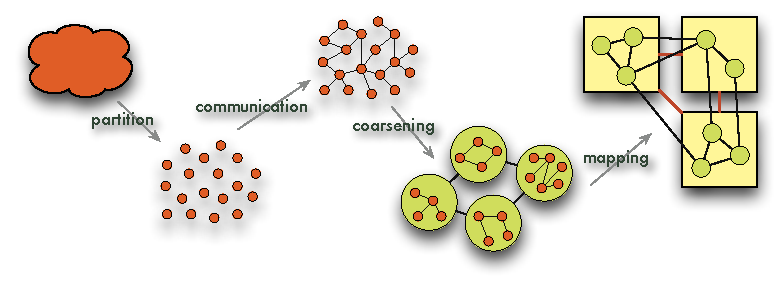
\includegraphics[scale=0.5]{figures/parallelization-steps.pdf}
      \label{fig:parallelization-steps-threads}
    \end{figure}
    \vspace{-1.75em}
%
    \begin{itemize}
    \item identify the work that can be done concurrently
    \item partition it in terms of work units, the fine grain tasks
    \item analyze the communication patterns among work units with an eye for critical sections
      and protecting shared data structures
    \item coarsen into threads, define the mutex categories and synchronization points
    \item let the OS schedule the threads onto physical processors
    \end{itemize}
%
  \item debugging threaded programs is very difficult
    \begin{itemize}
    \item preventing bugs through careful design is critical
    \item so is instrumenting the program to gain confidence in its execution
    \end{itemize}
%
  \end{itemize}
%
\end{frame}

% end of file 
